\begin{savequote}[8cm]
For generations, we have assumed that the efforts of mankind would leave the fundamental equilibrium of the world's systems and atmosphere stable. But it is possible that with all these enormous changes (population, agricultural, use of fossil fuels) concentrated into such a short period of time, we have unwittingly begun a massive experiment with the system of this planet itself.
  \qauthor{--- Margaret Thatcher}
\end{savequote}

\chapter{\label{ch:1-intro}Introduction} 

\minitoc

\section{Motivation}

In this section I justify photovoltaic materials research. First, the challenge we face as a human race -- global warming -- is introduced, followed by why we should take advantage of the sun as an energy source. The section ends with a discussion about the three generation of solar cell materials, and the inherent limitations of silicon solar cells.

\subsection{Energy use and global warming}

%The IPCC models have 5 things which need to happen in all scenarios. one of them is the reducition in energy output which we are doing. but must happen in conjunction with others.
Anthropogenic climate change is one of the greatest challenges we face as a human race and, as we have twelve years to limit climate change catastrophe, we are running against the clock. This viewpoint is not party political or the political hyperbole of the green left, as I have tried to allude to with the opening quote -- this is the current scientific understanding as established by the International Panel on Climate Change.\autocite{IPCC2018}

The story begins in the 18th century when the industrial revolution enabled unprecedented population growth, from 0.8 billion in 1750 to 7.5 billion in 2017.\autocite{Kaneda2017}
Industrial expansion combined with a growing population led to an exponential growth in the amount of coal and oil being burnt; between the years 1769 and 2006 there was an 800-fold increase in the world annual coal production.\autocite{MacKay2009}
Atmospheric \ce{CO2} concentrations increased as a result, leading to an increase in global temperatures, rising sea levels, and ocean acidification. The years 2014--2018 were the five hottest years on record \autocite{gistemp2018} and there has been a recent increase in extreme weather (heat waves, drought and floods) across the globe.\autocite{easac2018} Studies have shown that the probability of heat waves,\autocite{Black2016} wildfires\autocite{Abatzoglou2016} and flooding \autocite{Sweet2016,vanderWiel2017} have increased as a result climate change.

The threat of climate change seems not to have had a proportionate response from governments or many individuals. One reason for this is that changes in weather patterns are significant only when looked at over long time periods, and so it is difficult to communicate the risk carried by climate change. Another is that this is an inherently international problem, and that we do not have the political mechanisms in place to coordinate a global response. Despite the dramatic consequences of inaction, there seems to be little public appetite for changes which require a reduction in energy use. Instead there is a push towards technological solutions which may be able to reduce the negative effects of climate change without impacting upon our perceived quality of life.

%\begin{figure}[h]
%\centering
%  \includegraphics[width=0.5\columnwidth]{C01/figs/ag.png}
%  \caption[XKCD comic - climate change]{The XKCD comic character suggests that the timescales of climate change can lead to the perception that there is no climate change; like an electron an adiabatic potential, our environment changes and we simply adjust with it. Reproduced with permission from \url{https://xkcd.com/1321/}.} %like an electron under adiabatic, we may undergo a dramatic phase change without even being aware of it.
%  \label{xkcd}
%\end{figure}

%- 1979 : 1st world climate conference. 1990: 0.3 degree rise per decade, 1995: the balance of evidence suggests discenible huma influence on global climate. 1997 - kyoto protocol.

%- Toronto July 1988: Climate change is a serious challange, undertake actions to reduce, enhance research to reduce uncertainty.


%- 2015 : agreement to limit global temp to 2C or 1.5C if posible and net zero emissions by end of century

\subsection{The sun as an energy source}
One way to reduce the rate of climate change is to generate energy through processes that do not release net positive amounts of CO$_2$ into the atmosphere, and harnessing the vast amount of energy that is released from the sun is one way of doing this. This idea has been around for more than sixty years; in 1954 Bell Labs demonstrated that it was possible to convert sunlight into electricity by powering a small toy Ferris wheel and radio transmitter with a silicon solar cell. Reporting this event, The New York Times wrote:
%http://www.aps.org/publications/apsnews/200904/physicshistory.cfmthe New York Times wrote that:
\begin{displayquote}
“[the solar cell] may mark the beginning of a new era, leading eventually to the realization of one of mankind’s most cherished dreams–the harnessing of the almost limitless energy of the sun for the uses of civilization.”
\end{displayquote}
A solar flux density of $1361\,\textrm{Wm}^{-2}$ reaches the earth's atmosphere each second, which is almost $10^4$ times larger than any other external energy source.\autocite{Kopp2011} A quick back-of-the-envelope calculation shows that if we assume a sunlight to electricity conversion efficiency of 40\% (achievable using concentrated solar power) and zero transmission loss, we could meet the world's electricity demands ($22\,\textrm{PWh}$ in 2015\autocite{IEA2017}) by covering an area equivalent to Northumberland county ($5000\,\textrm{km}^2$) with photovoltaic solar panels.
%$46400\,Wm^{-2}$ is the absolute limit if we consider concentrator cell architectures (section \ref{SQlimit}). 
%
%The cost of PV installations is increasingly due to the infrastructure around the solar cell: for example, module encapsulation and installation\autocite{Green2016}. As a consequence, improving the efficiency of a device is the way to lower costs: with an increasing efficiency, a decreasing area is required to produce an equal amount of power, and all of the costs that scale with area are reduced. For new devices to succeed they must be able to match or exceed the efficiency of silicon.
However to harness this power we must be able to convert sunlight into electrical energy at a competitive price and at scale. Photovoltaic efficiency is key to price reduction as there are significant costs that scale with area,\autocite{Fraunhofer2015,Green2016} and a higher efficiency module can deliver the same energy for a smaller area.

The first photovoltaic devices could transform sunlight into electrical energy with an efficiency of around 6\%. The computing boom of the 1980s encouraged large investment into silicon research and  silicon cells with 20\% efficiency were reported in 1986.\autocite{Blakers1986} Since 1980 costs have decreased at an average rate of 10\% per year\autocite{Farmer2016} (Fig.\ \ref{module_price}) and the global market is growing, from a capacity of 1.9 GW in 2005 to 102 GW in 2016.\autocite{Jager-Waldau2017}

\begin{figure}[h]
\centering
  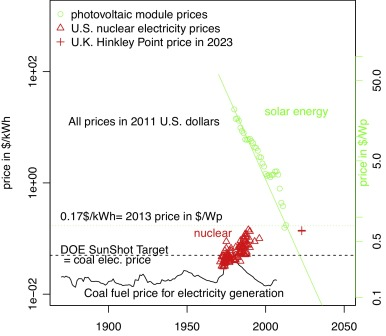
\includegraphics[width=0.6\columnwidth]{figures/ch1/solarcost.jpg}
  \caption[Historic and predicted costs of solar energy generation]{Historic and predicted costs of energy generation. The cost of solar energy (green) has been decreasing exponentially (at an average rate of 10\% per year) and is now comparable with the cost of energy generated from nuclear power (red). The dashed line corresponds to a  solar energy cost target from the US Department of Energy of \SI{0.05}{\$\per\kilo\watt\hour}. Reproduced with permission from the work of Farmer et al.\autocite{Farmer2016}}
  \label{module_price}
\end{figure}
% https://www.ise.fraunhofer.de/content/dam/ise/de/documents/publications/studies/AgoraEnergiewende_Current_and_Future_Cost_of_PV_Feb2015_web.pdf
% http://energy-age.blogspot.com/2015/02/pv-price-in-future.htmlf
% https://www.greentechmedia.com/articles/read/pv-solar-costs-have-fallen-10-per-year-since-1980#gs.HkfY3X4
% Schematic idea: GWP installed per year as a funnel (bottmoo 1980, top currrent) but also split into colour by material type. Shows growth in diversity as well as overall.
% the levelized cost of energy by PV has dropped dramatically: see schematic: WEF Renewable Infrastructure Investment Handbook
% https://openei.org/apps/TCDB/transparent_cost_database THIS IS A GREAT DATABASE FOR COMPARISON - use to generate own version of the schematic in WEF
%- 100MW in china is largest installed, top solar plants: http://www.pvresources.com/en/top50pv.php

In the UK the growth in renewable energy has led to a decreasing dependence on fossil fuels. The UK had it's first day without coal in 2017\autocite{Brown2017} and ran for three days without coal in 2018.\autocite{Vaughan2018} There appears to be a growing political will to take advantage of renewable energy; the first UK National Infrastructure Assessment recommends halting the development of nuclear power stations and diverting investment into solar and wind energy generation instead.\autocite{NIA2018} This switch away from nuclear energy is projected to be at no cost to the consumer.

It is widely predicted that solar power will continue to grow -- to what extent depends on the source: a recent study from Imperial College London estimates that solar power could supply 23\% of global energy demand in 2040.\autocite{Grantham2017} ExxonMobil, a company heavily invested in fossil fuels, predicts that all renewables combined will supply 20\% of global power generation in 2040.\autocite{exxon2018} Note that previous models have consistently underestimated the scale of photovoltaic deployment.\autocite{Creutzig2017}
 % - Future : looking to terawatt.  DOI: 10.1126/science.aal1288

\subsection{Beyond silicon: the need for new photovoltaic materials}

%- from library: Photovoltaic Solar Energy: From Fundamentals to Applications: Angèle Reinders, Pierre Verlinden, Wilfried van Sark, Alexandre Freundlich
Photovoltaic devices are commonly split into three generations. In this section I introduce each generation and discuss what is driving the development of new PV materials in a competitive market that is dominated by silicon.

\textbf{First generation}

The first generation devices are based upon mono- and poly-crystalline silicon wafers. They dominate the PV market; in 2016 90\% of total PV module production used this technology.\autocite{Jager-Waldau2017}. They are high efficiency (>20\%), reliable (25 year lifetimes) and low cost (<0.5 \$/W). There has been a steady decrease in cost due to i) device engineering improvements (eg: textured surfaces); ii) the economies of scale as silicon industrial processes are driven by a demand for computer chips; and iii) improved industrial practices which allow thinner and thinner wafers to be fabricated with less waste. However there are technological and physical limits to how much the cost of a crystalline silicon wafer can be reduced. First, the manufacturing process for silicon wafers is energy intensive and requires high temperatures. Second, silicon is an indirect bandgap material and as a result does not absorb sunlight efficiently; wafers have to be a minimum thickness ($\sim 60\mu \textrm{m}$) to compensate for this. It is difficult to reach this limit without snapping the material during fabrication as silicon is a hard and brittle material.

\textbf{Second generation}

Second generation devices are fabricated from the direct bandgap materials gallium arsenide (GaAs), cadmium telluride (CdTe), cadmium indium gallium diselenide (CIGS) and amorphous silicon (a-Si). These materials have higher absorption coefficients, so they can be built into lighter thin-film ($\sim 10\mu \textrm{m}$) architectures. A thin-film is not mechanically stable, it needs a substrate, but this opens up possibility of it being a flexible film.

CdTe was the first thin film to be commercialised and development has been led by the company First Solar, who have installed a total capacity of \SI{17}{\giga\watt}. Lifecycle assessments indicate that the CdTe energy payback time (the time required to generate as much energy as is consumed during production and lifetime operation of the system) is shorter than that of Si.\autocite{Koppelaar2017} However lower efficiencies are stifling the growth of this technology and there are also concerns about the elemental toxicity and scarcity. CIGS and a-Si each have a smaller market share than CdTe. High efficiency ($\sim 40\%$) GaAs devices have been developed for the high-value, low-volume space market.

% Much is invested into cheap solution deposition methods rather than expensive vacuum deposition like that used for GaAs. Jake Bowers / Mitzi
% What about GaInP??

\textbf{Third generation}

Third generation devices are emerging technologies which are not yet in the market. This includes organic and dye-sensitised materials, hybrid halide perovskites, and copper zinc tin sulfide (CZTS). These are abundant materials which can be fabricated through low-cost solution-deposition methods. Only the hybrid-halide perovskites have efficiencies high enough for commercialisation (currently 24.2\%).

For the third generation materials commercial success may come from opening up new markets rather than trying to compete directly with well established silicon technologies. For example, organic and hybrid perovskite technologies have tunable bandgaps and are being developed for semi-transparent building integrated photovoltaics.
There has also been recent research interest and commercial investment into silicon-perovskite single junction tandem cells.
%% DEFO need to expand this. Silicon has solved the PV problem pretty much. Perovskite needs to be stable, it potentially needs to NOT have lead (though actual environmental toxicity impact is low, legislation does not reflect this), and ideally a tunable (wider) bandgap.

%% all films more the 20% have been based on diamond. All FCC - even CZTS is double ZB. APART from perovskite!!

%%perovskite is basically comparable to silicon but stability is the issue. Needs to compete on price and efficiency.

%% PV is less than coal and gas in sunnier places

%% FAPI and CsPbI are not stable perovsite structure at RT, but by mixing large and small to get an average size you get a stable structure.

%% grain size of perovskite influences stability but not immediate efficiency.

%% should really emphasise the role of defects in degradation of the device.
%% MAPI has minimum toxicological impact. (plus compare to GaAs) - most comes from silicon. Pb is very scalable. 

%Inernational technology roadmap 2017 lays out growth in tandem cells. For a large market. This is the target. should be a perovskite module made in 2019.

%- http://www.sciencedirect.com/science/article/pii/S0306261917311339 : BIPV with perovskites
%-BIPV: functionalising buildings. Generating and storing energy. Make more than need: store in car which becomes a battery on wheels which then could feed into rest of house (people use car on average one hour per day). buildings as power stations - specific - low energy wireless device
%- This is what Dyesol company want to do. They are not going to compete with silicon on the arrays of solar farms. Going to look into market where silicon has not penetrated: where it cannot because of need to be solid single crystal. Aim is functionalisation of buildings with PV. Printing on steel.

\section{Key concepts in photovoltaics}

This section outlines the physical principles underlying solar cell operation, with a focus on carrier recombination. After introducing the key concepts and vocabulary, the design rules or ``wish list'' for a successful PV material are outlined. 
%Focus upon how we can design high-efficiency materials.

\subsection{Operating principles} \label{operatingprinciples}

% % use solar cat book images

A solar cell converts light into electricity through the following (simplified) process: i) a photon enters the device; ii) the photon is absorbed and creates an electron-hole pair in the absorber layer; iii) the electron and hole disassociate; iv) the electron and hole travel through the absorber layer to their respective contacts; v) the electron and hole are extracted to the external circuit to do electrical work.

\subsubsection{Device architecture}
The device architecture is determined by the properties of the absorber material. For example, in a hybrid halide perovskite material the photogenerated electron and hole are loosely bound to one another and thermal energy is enough to separate them. In this case, a planar $n$-$i$-$p$ architecture can be used, where $n$ is a n-type (electron-doped) material contacted to the cathode, $p$ is a p-type (hole-doped) material contacted to the anode and $i$ is the intrinsic (undoped) perovskite material (Figure\ \ref{SC_architecture}). In contrast, the photogenerated electron-hole pair in an organic solar cell is strongly bound. In this case, the electron-hole pair disassociate only at an interface and a mesoscopic architecture is used to facilitate this (Figure\ \ref{SC_architecture}). The conventional organic architecture is $p$-$i$-$n$, where the anode and p-type material are deposited onto the substrate first. The conventional architectures can be inverted to give $p$-$i$-$n$ junctions (for inorganic / hybrid absorber layers) or $n$-$i$-$p$ junctions (for organic absorber layers). In all cases, the n-type and p-type layers provide a built-in electric field that drives photogenerated electrons towards the cathode material and photogenerated holes towards the anode.
% pn junction sketch.
% see https://www-ssrl.slac.stanford.edu/content/science/highlight/2011-01-31/effects-thermal-annealing-morphology-polymer%E2%80%93fullerene-blends-organic and Late Stage Review pic
% an electron transport material (eg: TiO$_2$) acting as n-doped layer and a hole transport material (eg: Spiro-MeOTAD) acting as a p-doped layer.
% work function of p-type material is larer than work function of n-type material, and the charge carriers distribute so that the fermi level is continuous across the material.

\begin{figure}[h]
 \centering
   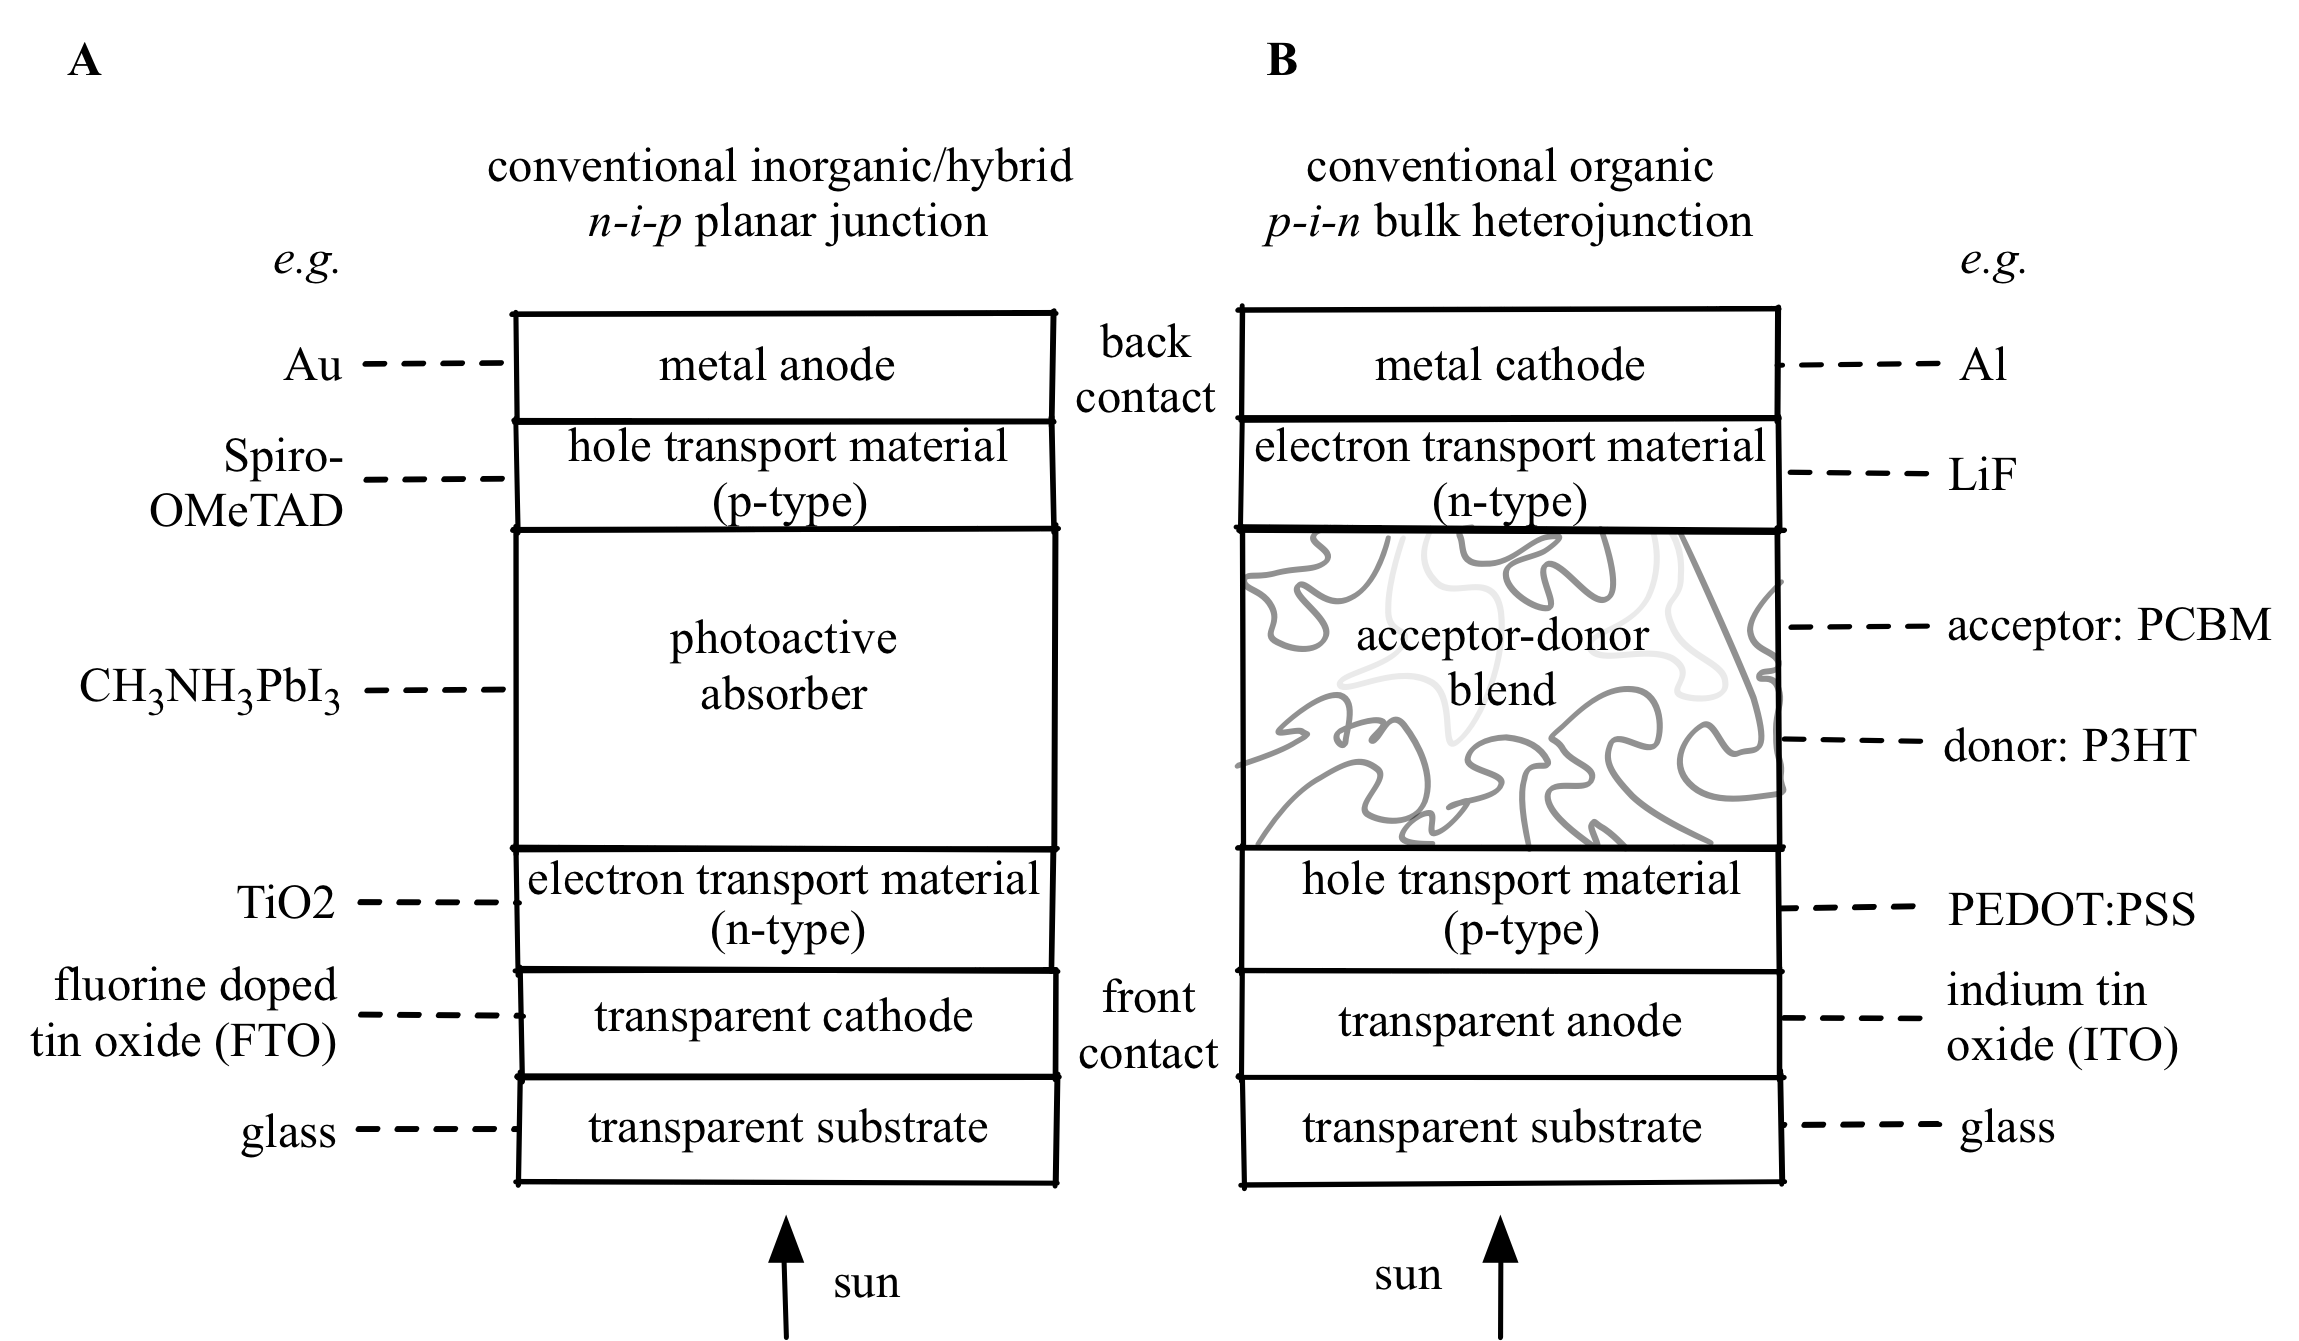
\includegraphics[width=1.0\columnwidth]{figures/ch1/PVarchitecture.png}
   \caption[Typical solar cell architectures]{(A) Schematic of the typical planar junction solar cell architecture used for an inorganic or hybrid material absorber layer (B) Schematic of the typical bulk heterojunction solar cell architecture used for an organic absorber layer. The mesoscopic architecture provides many interfaces where the electron-hole pair can disassociate.  In both cases there is a built-in electric field that drives photogenerated electrons towards the electron transport material and holes towards the hole transport material.}
   \label{SC_architecture}
 \end{figure}
% good info on organic cells here: https://www.sciencedirect.com/science/article/pii/S0038092X13003885

% %Can have multiple architectures for the same material.
% %Two types of device architecture used in commercial MAPI cells:
% % 2009: a perovskite dycell developed by miyasaka (liquid based DSSC architecture), 2013 planar thin film solid state solar cell by Snaith and graetzel( this showed standard semiconductors)
% %Planar (Snaith et al have dabs on it)
% %Mesoporous: which is said to be better re: hysterisis

%% could include here a section on "why does electrons flow toward n-type and holes towards p-type? include plot of band bending as a result of workfunctions in n-type and p-type materials and where the fermi levels are (near VBM ptype, near CBM -type) and the fact that the fermielvels must aligh.

Various strategies exist to increase device efficiency via device architecture engineering. For example, the current world record single junction silicon cell ($\eta=26.6\%$) has an additional wide bandgap material inserted between the absorption layer and contact material to reduce interfacial recombination, and interdigitated back contacts to reduce optical loss.\autocite{Yoshikawa2017} The most efficient solar cells ($\eta=46.0\%$) combine a multiple pn-junction (tandem) architecture with a lens to concentrate the incoming sunlight.

% %Adapting the device architecture can lead to large gains in efficiency. 
% % what have we learnt from Si
% %Buffer layers are used to 
% %- a lot of improvements come from tweaking the device:
% %- Inverted structures so defects do not proparagete.
% %- space layers and surface roughness to improve efficiency - engineering approaches
% %-  Remember most crriers generated near surface. Window is to stop carrier reaching surface

\subsubsection{Efficiency and reciprocity}
% %need to cite Nelson
For an external circuit with load $R$, a current $I$ and voltage $V$ is developed across the cell so that
\begin{equation}
    V = IR.
\end{equation}
$I$ and $V$ are related by a current-voltage curve (Figure\ \ref{current_voltage}).
A solar module operates at the maximum power point $P_m$, which is where the product of the voltage and current is maximum:
\begin{equation}
    P_\textrm{m}  = I_\textrm{m} V_\textrm{m}.
\end{equation} 
The open-circuit voltage $V_{\textrm{oc}}$ is the voltage produced when there is no contact to the external circuit (or, equivalently, the external circuit has an infinite load). 
The short-circuit current $I_{\textrm{SC}}$ is the current that flows when there is no load on the external circuit.
The fill factor FF is defined as:
\begin{equation}
    \textrm{FF} = \frac{I_\textrm{m}V_\textrm{m}}{I_\textrm{sc} V_\textrm{oc}}.
\end{equation}
The higher the fill factor, the higher the maximum powerpoint for a given $V_\textrm{oc}$ and $I_\textrm{sc}$.\autocite{Nelson2003} A fill factor of one would correspond to a current-voltage curve which is not \textit{actually} a curve, but a right angle.

 \begin{figure}[h]
 \centering
   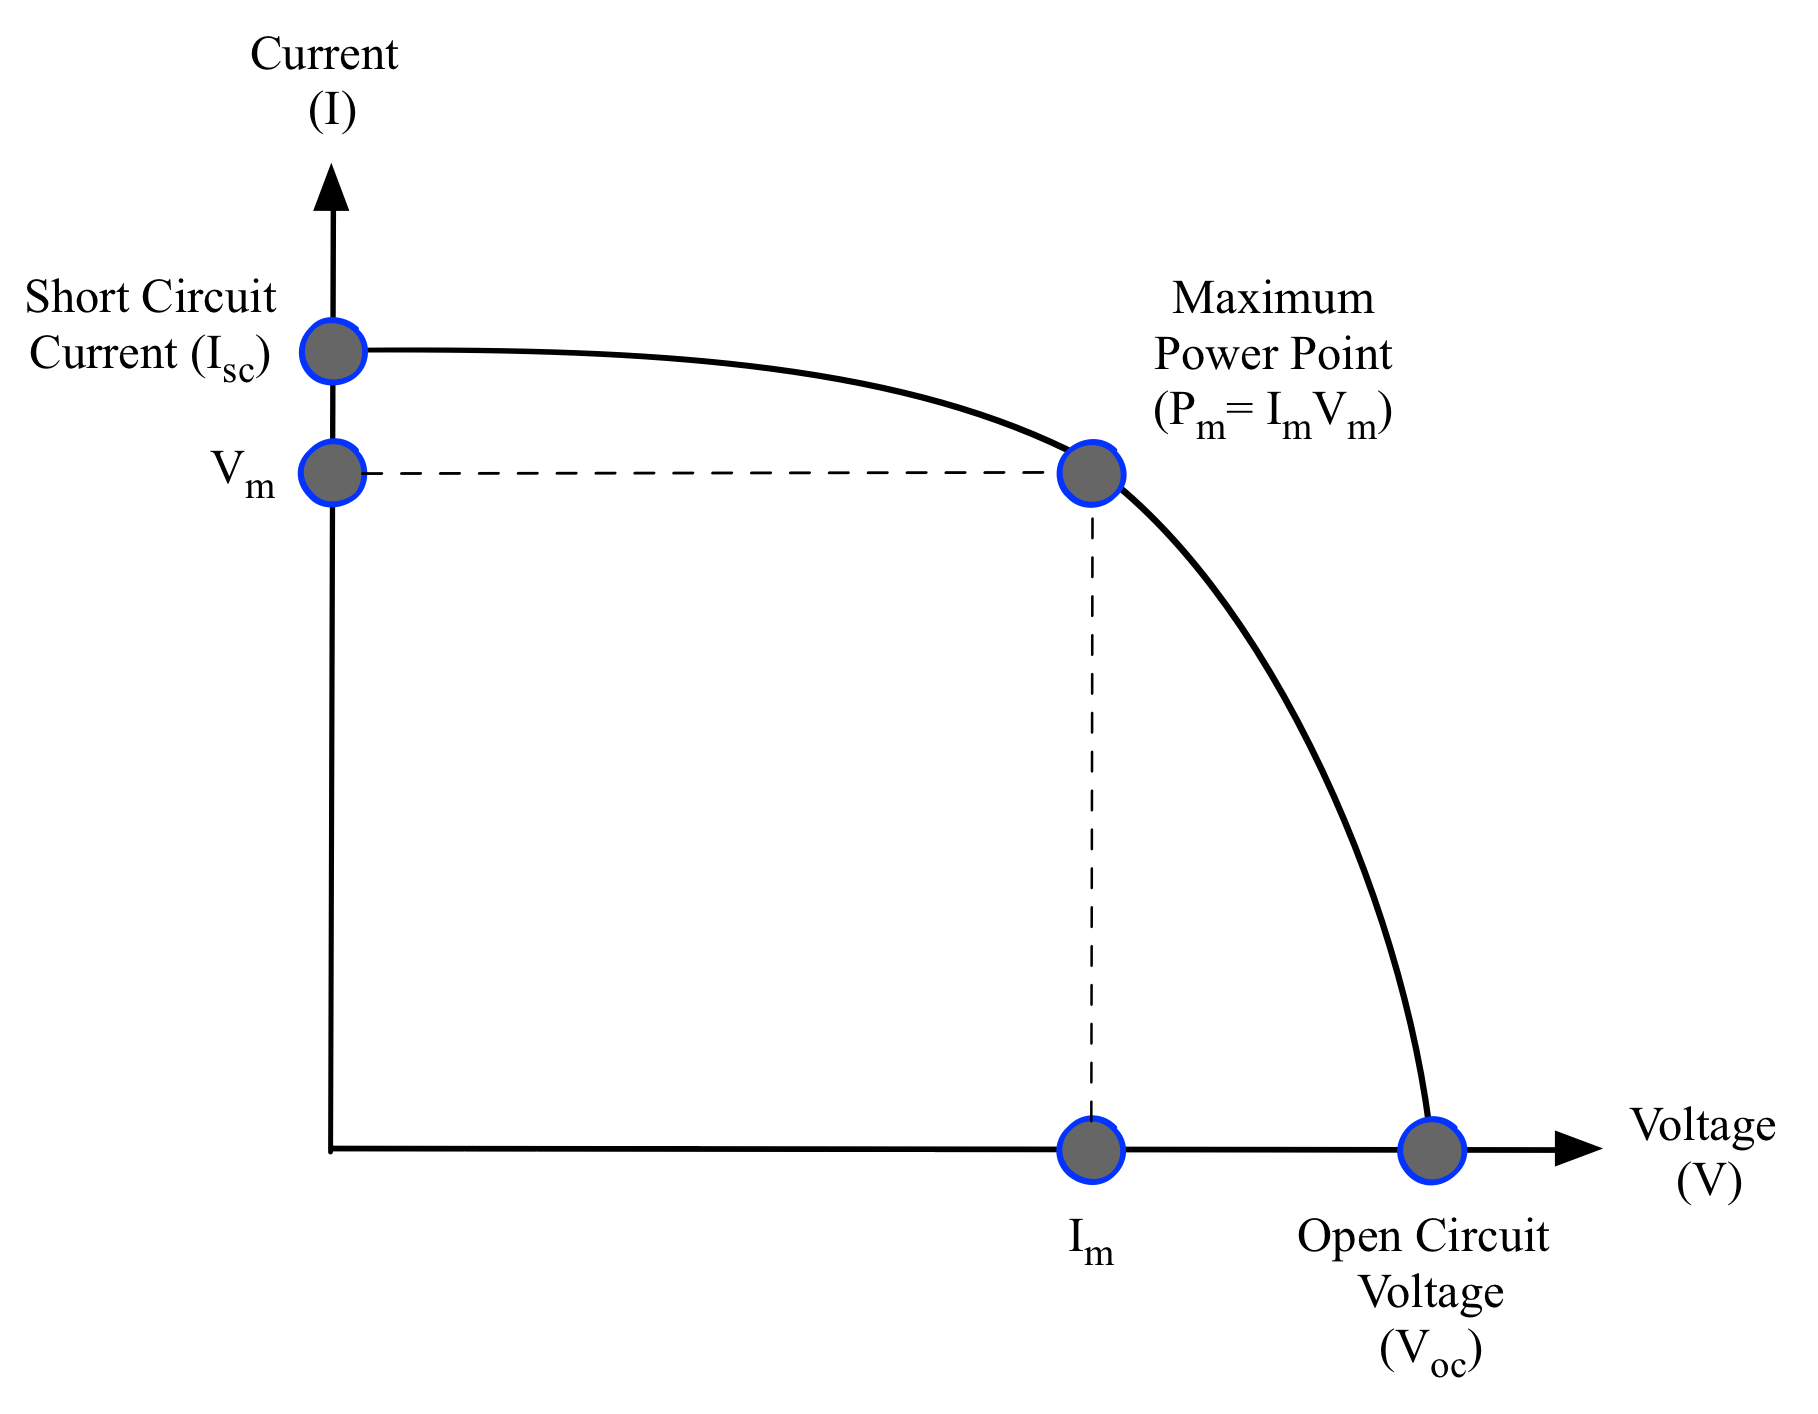
\includegraphics[width=0.65\columnwidth]{figures/ch1/current-voltage.png}
   \caption[Solar cell current-voltage curve]{Schematic of a current-voltage curve for a typical solar cell.}
   \label{current_voltage}
 \end{figure}

The efficiency $\eta$ of the solar cell under an incident light power of $P_\textrm{s}$ is given by
\begin{equation}
    \eta = \frac{P_\textrm{m}}{P_\textrm{s}} = \frac{I_\textrm{m} V_\textrm{m}}{P_\textrm{s}} = \frac{I_\textrm{sc} V_\textrm{oc} \textrm{FF}}{P_\textrm{s}}.
\end{equation}
Thus the three key figures of merit for a solar cell are the $V_\textrm{oc}$, $I_\textrm{sc}$ and FF, and these combine to give the efficiency $\eta$. 
However in all absorber materials there is a trade off between current and voltage; as the bandgap of a material decreases, more photons can be absorbed (higher $I_\textrm{sc}$) but the photogenerated charge carriers have less energy (lower $V_\textrm{oc}$).

%At short circuit, an efficient solar cell does not radiate any light as the excited electrons are extracted before radiative recombination is allowed.
At open circuit, all electrons and holes must recombine in the solar cell. In an efficient PV material the recombination is radiative as this is a thermodynamically unavoidable process via the energy level transitions needed for absorption. Non-radiative recombination, where the energy is dissipated as heat and eventually lost, is avoidable and should be minimised. For a fixed carrier concentration, a higher rate of photon emission corresponds to reduced non-radiative recombination; high radiative efficiency (as measured through e.g. electroluminescence) translates to high open circuit voltage.\autocite{Rau2007}
As a consequence of this reciprocity relation, we can predict the $V_\textrm{oc}$ and $I_\textrm{sc}$ from photoluminescence and photoconductivity studies respectively. This approach has been recently applied to hybrid halide perovskites.\autocite{Braly2018}
% %http://www.nature.com/articles/srep06071 and in Martin Green review for high efficiency PV: http://www.nature.com/nmat/journal/v16/n1/pdf/nmat4676.pdf
% %Also reciprocicty relation Uwe Rau: http://journals.aps.org/prb/abstract/10.1103/PhysRevB.76.085303.
% % Great discussion on this in perovskite review paper on Voc:  10.1002/aenm.201602358.

%plus the other nice paper previous link above I tink.

% %The below outlines how fermi level splitting as measured by PL can be used to predict Voc and JSc and it is applied to perovskties. https://pubs.acs.org/doi/pdf/10.1021/acs.jpclett.8b01152
% %Reciprocity meaning that IPCE and EQE-EL can determine the Voc: http://onlinelibrary.wiley.com/doi/10.1002/aenm.201400812/epdf.
% %ERE is the inverse of EQE and is easier to measure.
% %Can measure El and PL . EL on finished cells bus easier to measure well than PL.
% % $I_EL$ is prop to EQE (extension of reciprocity).
% %Nice description of ERE here: http://science.sciencemag.org/content/351/6280/1401.full
% %PL quantum yield

\subsubsection{The Shockley-Queisser limit}\label{sec:SQlimit}
The principle of detailed balance states that at equilibrium each microscopic process is balanced by its reverse process: for a photovoltaic device operating at open-circuit this means that the rate of photon absorption equals the rate of photon emission. Shockley and Queisser used the principle of detailed balance to calculate the maximum possible efficiency of a photovoltaic device\autocite{Shockley1961} (an alternative derivation is given in Ref. \cite{Nelson2003}). The PV efficiency is dependent upon the direct bandgap $E_g$ of the absorber material and the spectrum of the incident light. Assuming illumination under a standard AM1.5 solar spectrum, the efficiency can be plotted as a function of bandgap. For a single junction solar cell the maximum possible efficiency across is 33\%, which corresponds to an ideal bandgap of $\sim 1.4\,\text{eV}$ (Figure\ \ref{SQlimit}). 

\begin{figure}[h]
\centering
   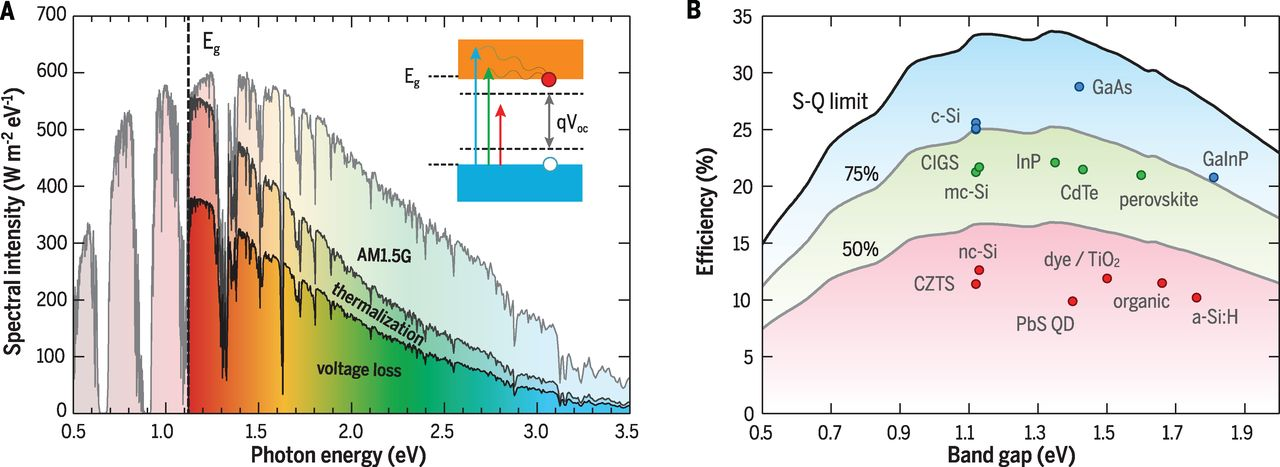
\includegraphics[width=1.0\columnwidth]{figures/ch1/SQlimit.jpg}
   \caption[AM1.5 spectral intensity and Shockley-Queisser efficiency]{(A) The AM1.5 spectrum. Photons below the bandgap are not absorbed, whilst energy is lost from above bandgap photons via carrier thermalisation. (B) The Shockley-Queisser efficiency of a single bandgap solar cell under AM1.5 illumination (thick black line). Also included are the top cell efficiencies for various PV materials. Reprinted with permission from the work of Polman et al.\autocite{Polman2016}}
   \label{SQlimit}
\end{figure}
%https://www.sciencemag.org/help/reprints-and-permissions

The model used to calculate the Shockley-Queisser limit is highly idealised. It assumes that all incident light is absorbed, that every absorbed photon creates an electron-hole pair, and that every electron is extracted to the external circuit. In real materials the absorption coefficient is not a step-function, and excited charge carriers can recombine through non-radiative processes before reaching the circuit. Only three materials have an efficiency above 75\% of the Shockley-Queisser limit: crystalline silicon (c-Si), GaAs and GaInP (Figure\ \ref{SQlimit}). Another metric, the spectroscopic limited maximum efficiency (SLME), accounts for absorption and emission characteristics and reduces the maximum theoretical efficiency.\autocite{Yu2012} For example, the candidate absorber material \ce{CuInS2} has a Shockley-Quiesser maximum efficiency of 33\% and SLME of 29\%.\autocite{Bercx2016} Non-radiative processes which contribute to the efficiency deficit will be discussed further in Section\ \ref{recombination}.

% %%discuss here Zunger SLME - where absorption is accounted for an it is not assumed to be a steo function.
% %% thermodynamic energy losses schematic https://www.nature.com/articles/nmat3263/figures/5

It is possible to exceed the Shockley-Queisser limit by challenging some of the assumptions built into the derivation. For example, the model assumes that once an electron is excited it will thermalise to the band edge, emitting the energy as phonons. This heat energy can no longer do useful work and results in a reduction of the $V_{\text{OC}}$. However `Hot carrier' cells, which extract electrons before they are able to thermalise, were successfully fabricated in 2014 (although it should be noted that they are currently limited to cryogenic temperatures and an incoming spectrum which is intense and monochromatic).\autocite{Hirst2014} 
%Intermediate band solar cells, where an electron recombines with a hole at band edge via a two-step process at a trap state, emitting two photons, have been suggested but have not been realised experimentally.

Another approach is to use tandem solar cells, where several absorber materials are stacked on top of each other. The materials are chosen to have complementary bandgaps, so that more of the solar spectrum can be absorbed with minimal thermalisation losses. GaAs-based four-junction tandem cells have reached an efficiency of 33\% and are used for space applications, though their uptake is limited by the costly wafer bonding method required for fabrication. The constraint of lattice matching -- that the strain at the interfaces must be minimised for device stability -- puts severe limitations on the material combinations which can be used for this approach. 

%Fundamental losses (LC Hirst diagram Prog Photovolt Res. Appl. 19 286 (2010). Carnot and emission is thermodynaics, unavoidable. Boltzmann is entropy (light from all directions, being emitted in one direction) but this can be changes with concentrator (light from all directions) or light only emitted one diection (?). Concentrators can take the form of mirrors (reflecivve) or lenses (refraction). Thermalisation and below Eg can be solved with multi-junctions, IBSC, hot-carriers, multi exciton generation. 


%Other assumptions and technologies which aim to work around this assumption are outlined in Table \ref{beating_SQ} 

% $$ Assumption | Solution | Challenges | Working device $$
% Single bandgap | Tandem solar cells | 
% Electrons will thermalise before being extracted to external circuit | Hot carrier solar cells | GaAs / quantum wells?
% Each photon generates a single electron | Intermediate band solar cells
% Boltzmann losses | concentrator PV | %


% schematic here

%Beating the SQ limit takes us from very basic physics to engineering.
%The SQ limit can be overcome by using solar concentrators (which is equivalent to not letting light escape) or by having an intermediate bandgap solar cell (see Jarv paper)
%- Concentrators: no boltzmann losses.
%- ALCHEMI project.
%- hot carrier solar cells. GaAs, Dimmock, 2014, progress in PV. cryogenic. intense, monochromic light. high risk / high reward.
%- It’s all about tandem solar cells (GaAs) for high value, niche market PV. The challenge is lattice matching. They have a 4J 33\% GaAs for space application. Fabricated using MBE/MOVPE (more expensive).
%- Ratchet route – intermediate band solar cell – requires that the intermediate band does not become a place for recombination which can happen when introduced as a defect band as is usually done (can’t be single defect state: wont be able to build up considerable charge)
%Hot carrier has potential to make huge gains. But incredible tight material specification. Needs to be incredibly physically thin.
%Multijunction cells are great. Boltzmann loss increases but there are gains re: thermalisation and bandgap losses (louis hirst paper). Problem is lattice matching the MJ cells. Wafer bonding allows different attice parameters but is costly: there is always a trade.
%Spectral splitting. Interstitial light trapping.
%- New architectures: tandem etc. 33\% reached:https://www.nature.com/articles/s41560-018-0125-0
%- Concentrated PV is used to offset the cost of
%- multijunctuion PV.
%- Lattice matching in PV is problematic esp. over a range of temperatures. MOVCD iii-v on Si. Quantasol

%for polycrystalline:. Bryan huey - nanoscale tomography of photocarrier transport in operating CdTe solar cells. The AFM technique allows to map the PV properties (I-V, Isc, Voc) with high spatial resolution so we see that the Isc and Voc couple to the microstructure.

%Following the work of Hirst et al., the 
%- ned edkins dauke publications about different types of loss. Loise Hirst, progress in PV. Lovely schematic from 2011: Louise hirst: fundamental loss in solar cells, progress in PV. Carnot and emission is thermodynaics, unavoidable. Boltzmann is entropy (light from all directions, being emitted in one direction) but this can be changes with concentrator (light from all directions) or light only emitted one diection (?). Concentrators can take the form of mirrors (reflecivve) or lenses (refraction). Thermalisation and below Eg can be solved with multi-junctions, IBSC, hot-carriers, multi exciton generation. 
%- this is related to the unavoidable thermodynamic losses due to entropy (see Ross). PLQY can be used to give us the quasi fermi level splitting.
%- about thermodynamic losses: good review: https://journals.aps.org/prb/abstract/10.1103/PhysRevB.90.035211

\subsection{Carrier recombination} \label{recombination}
Electron-hole recombination competes with charge extraction to the external circuit, and as such it is a well examined process. Three pathways for electron-hole recombination are outlined in Figure\ \ref{recombination_processes}. During radiative recombination the electron directly recombines with a hole to produce a photon and, in the case of indirect recombination, phonons. This recombination channel is unavoidable in PV devices as the same channel is used for light absorption. The second pathway, Shockley-Reed-Hall (SRH) recombination, is a two step process mediated via a trap state. In PV devices this pathway should be minimised as the kinetic energy of the electron and hole is transformed to vibrational energy (phonons) and cannot be used for useful work. The third pathway, Auger recombination, is also a non-radiative process. Here the electron directly recombines with a hole, and the resulting energy and momentum is transferred to another conduction band electron.
% %4.4x10^18 is auger recombination in MAPI - see Tom hopper work when it comes out.

\begin{figure}[h]
 \centering
   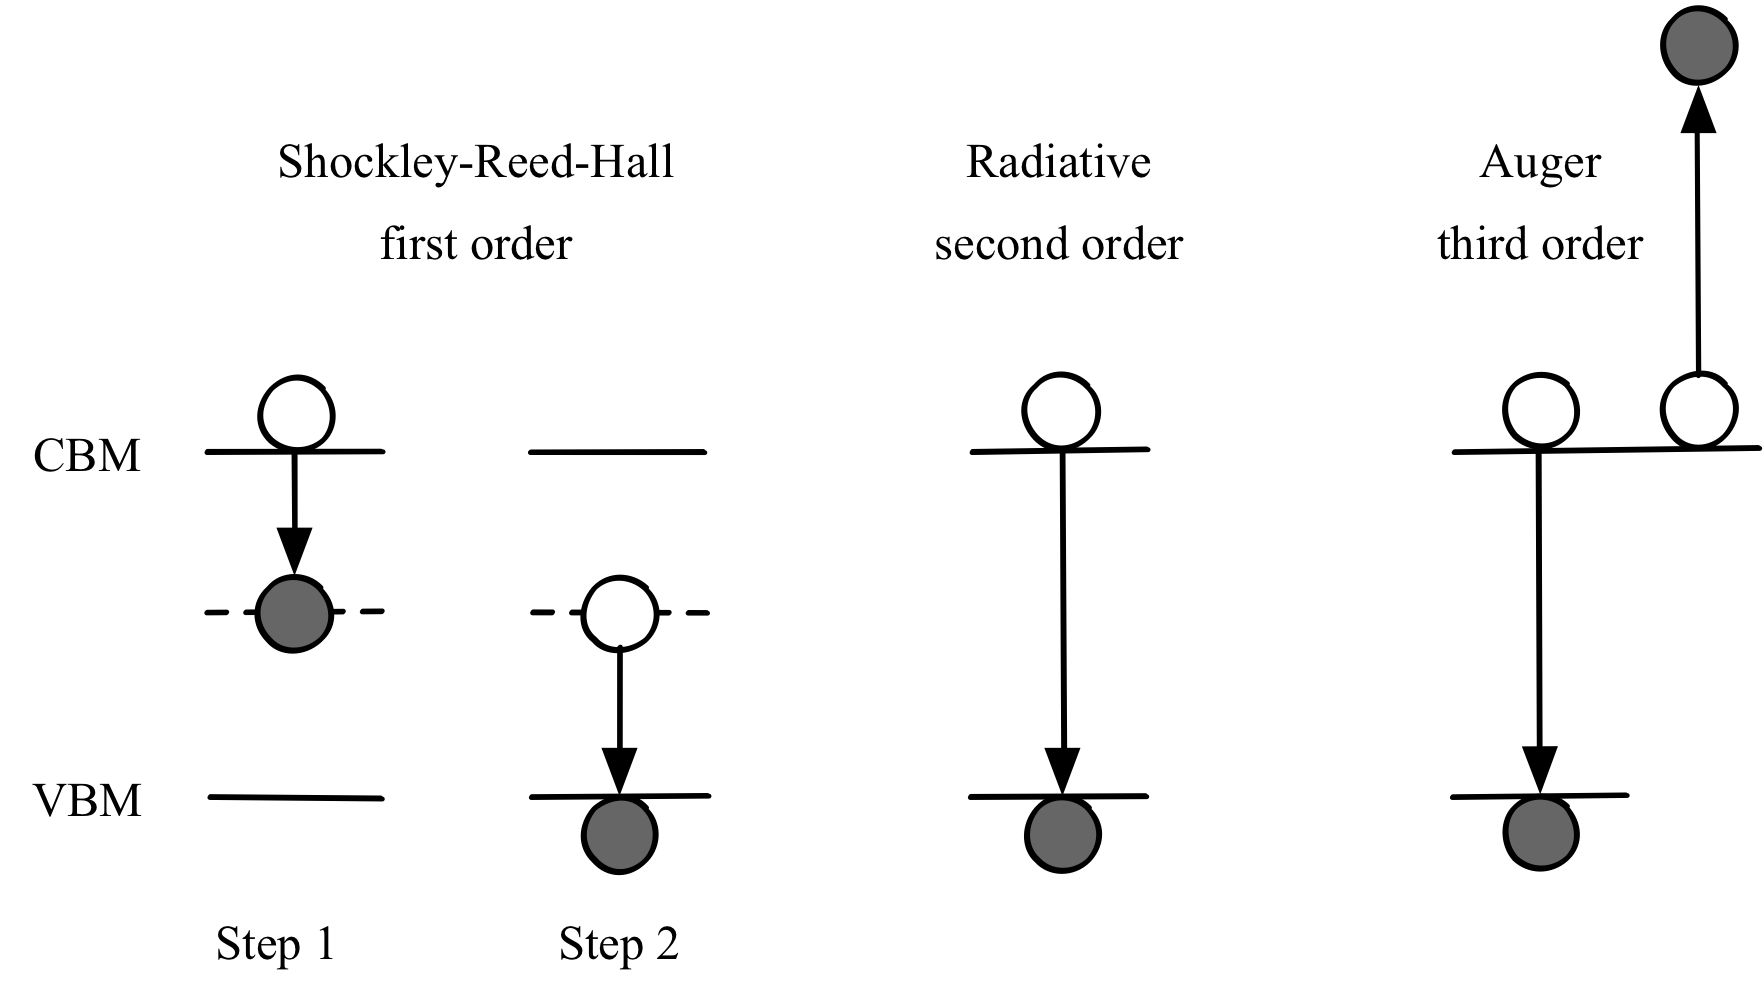
\includegraphics[width=0.65\columnwidth]{figures/ch1/recombination.png}
   \caption[Electron-hole recombination pathways]{A schematic of the three possible electron-hole recombination pathways. In each case, an electron at the conduction band minimum combines with a hole at the valence band maximum. First-, second- and third-order processes correspond to one, two and three particle processes respectively.}
   \label{recombination_processes}
 \end{figure}

Radiative recombination and Auger recombination are unavoidable processes intrinsic to the material, whereas SRH recombination is an avoidable process that can be controlled through defect engineering. The SRH recombination rate is given by
\begin{equation}
U_\textrm{SRH} = \frac{np-n_\textrm{i}^2}{\tau_\textrm{n,SRH}(p+p_t)+\tau_\textrm{p,SRH}(n+n_t)},
\end{equation}
where $n$ ($p$) is the density of electrons (holes), $n_i$ is the intrinsic carrier density and $n_t$ ($p_t$) is the value of the electron (hole) density when the electron Fermi level is equal to the trap level $E_t$: 
\begin{align}
n_t &= n_ie^{\frac{(E_t-E_c)}{k_BT}} \\
n_p &= n_ie^{\frac{(E_v-E_t)}{k_BT}},
\end{align}
where $E_c$ and $E_v$ are the energies of the CBM and VBM respectively. The recombination rate has a maximum when the rates of hole capture and electron capture are comparable. This happens when the trap level is in the middle of the bandgap, and $n_t = p_t$. % note here that deep state not needed: czts : https://pubs.acs.org/doi/pdf/10.1021/acsenergylett.7b01313

$\tau_\textrm{n,SRH}$ ($\tau_\textrm{p,SRH}$) is the electron (hole) lifetime. For a trap density $N_t$, mean thermal electron (hole) velocity $v_n$ ($v_p$) and electron (hole) capture cross section $\sigma_n$ ($\sigma_p$), the lifetimes can be approximated as 
\begin{align}
\tau_\textrm{n,SRH} &= \frac{1}{v_n\sigma_nN_t} \\
\tau_\textrm{p,SRH} &= \frac{1}{v_p\sigma_pN_t}.
\end{align}
The standard approach for calculating the trap density from first principles is give in Chapter\ \ref{ch:3-methods}, and a method for calculating the capture cross section is outlined in the results Chapter\ \ref{ch:6-defects}.

\subsubsection{Experimental measurements of recombination rates} \label{exprecombo}

Carrier lifetimes and recombination rates are difficult to measure experimentally as ultra fast optical and electronic sensors are needed to capture transient behaviour, and this must be done in conditions relavant to photovoltaic performance. Time resolved photoluminscence (TRPL) and photoconductivity measurements are used to infer the recombination rates for each recombination pathway.
Each pathway scales differently with carrier concentration, as specified by the following rate equation:
\begin{equation}
\frac{d n}{\d t} = G -k_1n -k_2n^2 -k_3n^3 
\end{equation}
where $G$ is the rate of electron-hole generation, $k_1$ is the rate constant for SRH recombination, $k_2$ is the rate constant for radiative recombination and $k_3$ is the rate constant for Auger recombination. SRH recombination via a trap state is a one particle process that scales linearly with the carrier concentration. Radiative recombination is a two particle process that depends on the electron density ($n_e$) and hole density ($n_h$), so scales quadratically with carrier concentration. Auger recombination requires three particles and scales cubically.
TRPL uses short laser pulses to excite excess electrons and holes which then decay via recombination or carrier extraction at an interface. Exponential curves are fitted to the TRPL signal at different laser fluences to extract carrier lifetimes. In general, for solar cells operating under 1.5AM illumination, second order SRH recombination is the dominant recombination mechanism.
% 
% https://www-herz.physics.ox.ac.uk/publications/Herz16a.pdf
% https://aip.scitation.org/doi/10.1063/1.4891595
% https://www.nanoge.org/proceedings/ABXPV/58c15c889c168f501d8b9aa2


 \subsection{Design principles for absorber materials}
 
Solid state physics and computational chemistry can connect microscopic material processes to macroscopic observables. The tools of each field have been applied to a range of inorganic and organic materials, and have successfully explained the observed properties of existing materials.
There is also a more recent approach to materials science called ``inverse design''. This is where the desired functionality of a new material is stated first, and computational tools are used to predict which materials will exhibit such features.\autocite{Zunger2018}
The hope is that this approach will improve upon discovery by trial and error, and accelerate the design of new materials.
%Previous technologically important material properties were discovered by trial and error (e.g. superconductivity, giant magneto resistivity);

High-throughput computational screening is a brute force approach to inverse design. Here, an automated procedure calculates a set of properties across a large number of atomic structures. This approach has been used to identify battery electrolytes,\autocite{Qu2015} organic photovoltaic materials\autocite{Hachmann2011} and materials for carbon capture and storage,\autocite{Dunstan2016} amongst others. 
Materials screening criteria must be defined so that successful materials are identified and selected for further study. Some criteria are easy to identify - for example the thermodynamic stability, which ensures that the material is synthesisable. This criteria can be expanded to include the features found in existing successful materials. For example, hybrid halide perovskites are defect tolerant - they contain a low concentration of defects which are detrimental to opto electronic performance. The electronic parameters which underpin the defect tolerance of hybrid halide perovskites have been identified so that they may be used to screen for new defect-tolerant materials.\autocite{Brandt2015} 
% https://pubs.rsc.org/en/content/articlelanding/2016/EE/C5EE03253A#!divAbstract
% https://pubs.acs.org/doi/10.1021/jz200866s
% https://perssongroup.lbl.gov/papers/compmatsci2015-electrolytegenome.pdf

With the concept of inverse design in mind, items for a successful PV material ``shopping list'' are listed below. The final three items (toughness, elemental abundance, elemental non-toxicity) are not necessary for successful devices in the lab, but would promote commercialisation of the technology.


\textbf{Thermodynamic stability}

The material should be thermodynamically stable with regard to competing phases so that it does not degrade over years of operation. The binary compound CdTe was the first thin film PV material to be commercialised and, similar to GaAs, it has no competing phases. Quaternary chalcogenide compounds such as \ce{CISSe} and CZTS have many more competing phases to consider and the chemical potentials during synthesis must be very finely tuned for stability, which hinders their development.
% Cu3Bi5S3 chalcogenide (major group). 0.1\% efficiency. Probelm: other phases. Keep it cimple: Sb2S3/Sb2Se3 - 5.5% with 3o papers/
%The same thing that makes a material have a good bandgap is that which makes it degrade (something about the bonding strenght??)


\textbf{Optimum bandgap}

Ultimately, it is the spectrum of the sun and features of our atmosphere (light scattering and absorption) that dictates the design of solar cells; we must optimise our solar technology to take advantage of the spectrum that is particular to our planet. The Shockley-Queisser limit, discussed in subsection\ \ref{sec:SQlimit}, gives an optimum bandgap of \SI{1.4}{\electronvolt}.\autocite{Ruhle2016}
Atomic disorder or point defects can reduce the material band gap. Quaternaries with elemental species of a comparable atomic radii are more likely to exhibit atomic disorder -- for example in CZTS this leads to a bandgap reduction of \SI{30}{meV}.\autocite{Rey2018}


\textbf{Strong light absorption}

The absorption coefficient specifies how much light of a particular wavelength is absorbed by a material. Different semiconductor materials have different absorption coefficients; those with a higher absorption coefficient will more readily absorb light. Silicon is an indirect bandgap material that requires phonon-assisted absorption. As a result, crystalline silicon absorbs 92\% of light in a thickness of  \SI{200}{\micro\metre}, whilst CdTe can absorbe the same amount in a thickness of \SI{1}{\micro\metre}.\autocite{Poortmans2006}
%As a result of relativistic spin-orbit coupling, the hybrid halide perovskite MAPI is also an indirect bandgap material. However, as spin splitting of the conduction band edge is small () and the density of states at the valence band edge is large, this has a negligible influence on light absorption in the material.\autocite{Azarhoosh2016}


\textbf{Low exciton binding energy}

After light absorption, a bound electron-hole pair (exciton) is created. The electron and hole must disassociate so that they can travel to their respective contacts. Here, the dielectric response is key, as this determines how readily a material will screen electrostatic perturbations. Organic solar cell materials are limited by low dielectric constants ($\epsilon_0 \approx 3--4$) that lead to large exciton binding strengths.\autocite{Brebels2017} In inorganic or hybrid materials the dielectric constants are higher ($\epsilon_0=10.4$ for CdTe,\autocite{Madelung2004} whilst values vary from $\epsilon_0=16.6$ to $\epsilon_0=28.5$ for MAPI\autocite{Wilson2019}).
% dielectric constant - effective mass theory
% polar domains for charge separation


\textbf{High carrier mobility}

Some materials may have suitable optical properties but are unable to transport the photogenerated charge efficiently to the contact layers. Carrier mobility quantifies how quickly an electron or hole can move through a material when pulled by an electric charge. 
Light carrier effective masses (high band dispersions) correspond to higher mobilities. However light effective masses are not sufficient in themselves as there are various scattering channels to consider: lattice scattering, carrier-carrier scattering and defect scattering. The most significant scattering mechanisms in a PV material are lattice scattering and ionized defect scattering.
A high dielectric constant is beneficial to carrier mobility as the rate of ionized defect scattering is proportional to $\frac{1}{\epsilon^2}$. The composition of the material is also important -- for example, vacancies in gallium nitride (Ga($3+$)N($3-$)) carry a larger charge and have a larger scattering cross section than vacancies in MAPI ($CH_3NH_3$($1+$)Pb($2+$)I($1+$)$_3$).


\textbf{Long carrier lifetime}

Carrier lifetime has already been discussed in the context of electron-hole recombination in Section\ \ref{recombination}. Whereas the concentration of defects is important for carrier mobility, here it is the energy of defect states with respect to the valence and conduction band which is important. This is discussed in Chapter \ref{ch:6-defects}. In summary, the key is to minimise non-radiative recombination via deep level defect states (also known as ``killer defects''). Carrier diffusion length, another important figure of merit with regard to carrier transport, is proportional to the product of carrier mobility and lifetime.


\textbf{Compatibility}

For efficient charge extraction, the PV absorber layer must be compatible with suitable contact and/or buffer layers. Firstly, the energy levels of the interfacing materials must align so that there is an electrical potential gradient to extract the charge, without significant loss of $V_\textrm{OC}$. For example, band mis-alignments are reported to be the source of poor photovoltaic efficiencies in the candidate absorober materials \ce{BiSI} and \ce{BiSeI}.\autocite{Ganose2016} Secondly, lattice mismatch at the interface should be avoided as this can lead to deep point defects that provide sites for non-radiative recombination and, in the case of more severe strain, an incoherent interface with many defect sites and weak chemical bonding. Computational screening procedures can be used to identify potential electronically and structurally matched contact layers and this has been recently applied to the hybrid halide perovskites.\autocite{Butler2016}
%more examples?
% http://science.sciencemag.org/content/sci/352/6283/aad4424.full.pdf “Photovoltaic materials: Present efficiencies and future challenges”


\textbf{Toughness}

Silicon is a brittle material; the majority of Si material in a solar cell is used as a mechanical carrier to prevent crack propagation, and glass must be used as a protective layer. The resulting cell is often too heavy to be installed on structures which are made from wood or sheet metal. In addition, the bulk of system costs are higher for heavier cells. Organic photovoltaics, and to some extent perovskites, are tougher and can be made using roll-to-roll print processes onto a flexible substrate.


\textbf{Elemental abundance}

The power generated from PV installations must exceed \SI{1}{TW} to make a real impact on global carbon emissions.\autocite{Battersby2019} To meet this demand, PV materials must be made from abundant elements that are in ready supply at reasonable cost. To quantify this criteria, the Herfindahl–Hirschman index (HHI), which is used in economics as a measure of market concentration, can be applied to elements. The HHI indicates that Si is abundant but that production is highly concentrated in a few countries. Elements common to the third generation of materials---Cu, Zn, S, Se, Sn---are less abundant but their production is more highly distributed across the globe.\autocite{Gaultois2013}


\textbf{Elemental non-toxicity} 

Finally, toxic elements may hinder the succesful commercialisation of future PV technologies. The problem is not insurmountable; cadmium telluride is toxic if ingested but is a commercial solar cell material. Encapsulation and recycling can reduce any risk, but add another level of complexity to the development of new solar technologies.

\section{Summary}

% need to point out that the highest efficiencies are from single crystal silicon and GaAs 26-29 mark. Lower cost polycrystalline in 20-23 mark. http://science.sciencemag.org/content/sci/352/6283/aad4424.full.pdf
To reduce the rate of climate change we must decrease our reliance on fossil fuels, and increasing the proportion of photovoltaic energy is one way to achieve this. This may only be politically feasible if the costs associated with PV energy can continue to exponentially decrease. As the well-established silicon technologies are limited by high capital expenditures, there is an incentive to develop new low-cost, high-efficiency and reliable technologies. Flexible thin-film architectures also allow for expansion into the new market of building integrated photovoltaics. Currently no material has met these requirements,\autocite{Zakutayev2017} although promising performance from emerging technologies such as the hybrid halide perovskites motivates further research.
% - start with what needed in general then what needed material properties wise to deliver this.
% - defects run throughout this chapter:
% - Defects can be fatal and vital : (good chapter quote?): Defects in Semiconductors: Some Fatal, Some Vital Hans J. Queisser* and Eugene E. Haller 
% - Ability to accelerate the design of PV materials through computation. Growth in computational tools (web of science keyword search), accesibility to non-specialists

% - light management vs carrier management. engineering vs basic science.

% Learn from the Si community: passivate the grain boundaries, specific and controlled doping, improve material quality, bandgap grading.
% Seen a 
% Wish list of properties.

% Key themes in this work: SRH.

\section{Thesis outline}

Organic-inorganic halide perovskites, the subject of this thesis, present a number of challenges for first-principles atomistic materials modelling. These `plastic crystals' feature dynamic processes across multiple length-scales and time-scales, which include mixed ionic-electronic transport, highly anharmonic lattice dynamics and strong relativistic (spin-orbit coupling) effects on the electronic band structure.
These issues, which affect the operation of solar cells, are outlined in the following chapter. 
This is followed by a brief introduction to the theory that underlies almost all of the work in this thesis - Density Functional Theory (DFT). 
To model an imperfect material (one with crystal defects), or temperature effects, a series of post-processing steps must follow the DFT calculation. These are also outlined in Chapter Three.

Chapters Four--Six contain the thesis results. Each results chapter also contains any additional theory where required and calculation steps.
Bulk transport and optical properties of the perfect material are calculated using Effective Mass Theory (EMT) in Chapter Three. 
EMT often assumes a parabolic electronic band dispersion, in this chapter distortions away from parabolicity are considered.
Temperature effects are introduced in Chapter Four. 
At room temperature the inorganic octahedral \ce{PbI3} units tilt back and forth, and the coupling strength between this tilting and the electronic sub-sytem is quantified.
Point defects are introduced to our model in Chapter Six. Point defects can be benign or harmful to device performance, depending upon the properties of the defect. This chapter reports the properties of the iodine interstitial point defect.


